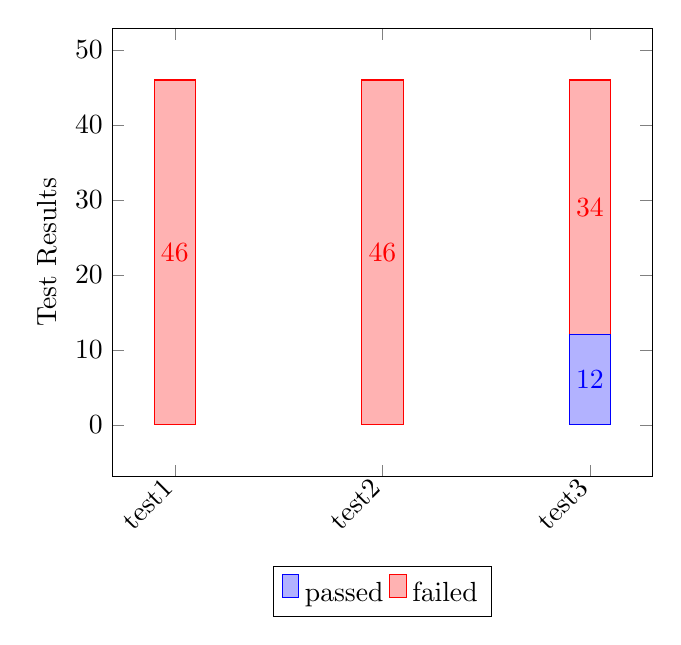
\begin{tikzpicture}
\begin{axis}[
    ybar stacked,
	bar width=15pt,
	nodes near coords,
    enlargelimits=0.15,
    legend style={at={(0.5,-0.20)},
      anchor=north,legend columns=-1},
    ylabel={Test Results},
    symbolic x coords={test1, test2, test3},
    xtick=data,
    x tick label style={rotate=45,anchor=east},
    ]
    \addplot+[ybar] plot coordinates {(test1,0) (test2,0) (test3, 12)};
    \addplot+[ybar] plot coordinates {(test1,46) (test2,46) (test3, 34)};
\legend{\strut passed, \strut failed}
\end{axis}
\end{tikzpicture}
